\documentclass[border=10pt]{standalone}
\usepackage[svgnames]{xcolor}
\usepackage{amsmath}
\usepackage{pgfplots}
\pgfplotsset{compat=newest}
\usepackage[sfdefault]{FiraSans}
\usepackage{FiraMono}
\renewcommand*\familydefault{\sfdefault}
\begin{document}
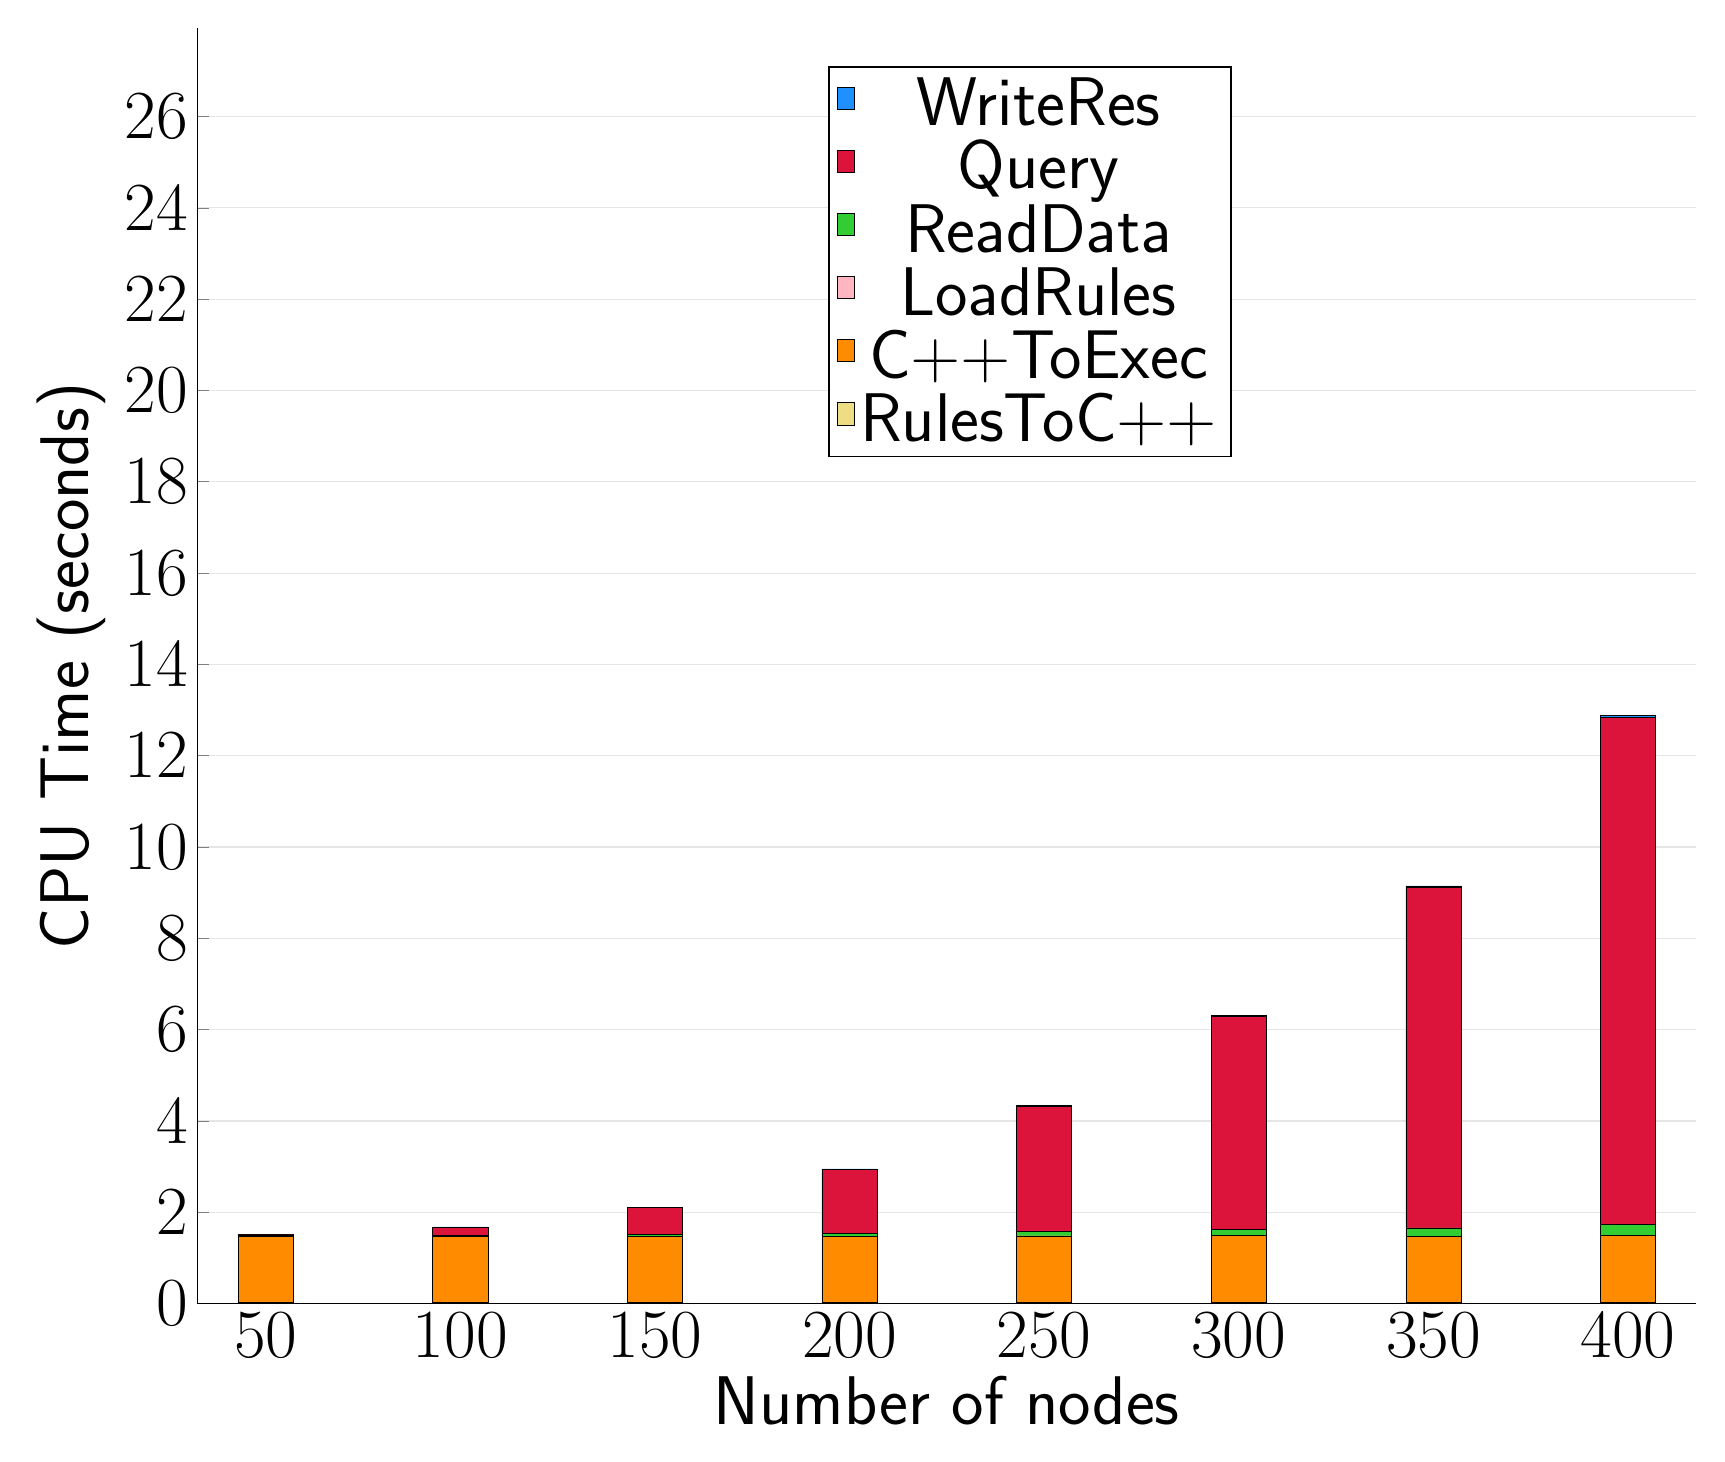
\begin{tikzpicture}
	\begin{axis}[
			ybar stacked,
			width=1.7\textwidth,
			bar width=0.7cm,
			ymajorgrids, tick align=inside,
			major grid style={draw=gray!20},
			xtick=data,
			ymin=0, ymax=27.933910000000004,
			axis x line*=bottom,
			axis y line*=left,
			enlarge x limits=0.05,
			legend style={
					at={(0.69, 0.97)},
					anchor=north east,
					legend columns=1,
					font=\Huge,
				},
			ylabel={CPU Time (seconds)},
			xlabel={Number of nodes},
			label style={font=\Huge},
			tick label style={font=\Huge},
		]
		\addlegendimage{fill=DodgerBlue, draw=black, line width=0.2pt}
		\addlegendentry{WriteRes}
		\addlegendimage{fill=Crimson, draw=black, line width=0.2pt}
		\addlegendentry{Query}
		\addlegendimage{fill=LimeGreen, draw=black, line width=0.2pt}
		\addlegendentry{ReadData}
		\addlegendimage{fill=LightPink, draw=black, line width=0.2pt}
		\addlegendentry{LoadRules}
		\addlegendimage{fill=DarkOrange, draw=black, line width=0.2pt}
		\addlegendentry{C++ToExec}
		\addlegendimage{fill=LightGoldenrod, draw=black, line width=0.2pt}
		\addlegendentry{RulesToC++}
		\addplot +[fill=LightGoldenrod, draw=black, line width=0.2pt] coordinates {
				(50, 0.030000000000000006)
				(100, 0.030000000000000006)
				(150, 0.030000000000000006)
				(200, 0.030000000000000006)
				(250, 0.030000000000000006)
				(300, 0.030000000000000006)
				(350, 0.030000000000000006)
				(400, 0.030000000000000006)
			};
		\addplot +[fill=DarkOrange, draw=black, line width=0.2pt] coordinates {
				(50, 1.4409999999999996)
				(100, 1.4429999999999998)
				(150, 1.4489999999999998)
				(200, 1.4439999999999995)
				(250, 1.454)
				(300, 1.456)
				(350, 1.446)
				(400, 1.4649999999999999)
			};
		\addplot +[fill=LightPink, draw=black, line width=0.2pt] coordinates {
				(50, 9.939999999999999e-05)
				(100, 0.0001204)
				(150, 7.2e-05)
				(200, 0.0001075)
				(250, 8.300000000000001e-05)
				(300, 6.850000000000001e-05)
				(350, 0.00010660000000000002)
				(400, 0.0001111)
			};
		\addplot +[fill=LimeGreen, draw=black, line width=0.2pt] coordinates {
				(50, 0.0055095000000000005)
				(100, 0.019796200000000007)
				(150, 0.0382915)
				(200, 0.06571160000000001)
				(250, 0.09608249999999999)
				(300, 0.133866)
				(350, 0.18132189999999998)
				(400, 0.23513540000000002)
			};
		\addplot +[fill=Crimson, draw=black, line width=0.2pt] coordinates {
				(50, 0.0304541)
				(100, 0.18330929999999998)
				(150, 0.5892850999999999)
				(200, 1.401393)
				(250, 2.735742)
				(300, 4.6695530000000005)
				(350, 7.457388000000002)
				(400, 11.11469)
			};
		\addplot +[fill=DodgerBlue, draw=black, line width=0.2pt] coordinates {
				(50, 0.0009644999999999999)
				(100, 0.0028721)
				(150, 0.006373800000000001)
				(200, 0.011119600000000002)
				(250, 0.017543)
				(300, 0.024711100000000003)
				(350, 0.0339666)
				(400, 0.044408199999999995)
			};
	\end{axis}
\end{tikzpicture}

\end{document}
